\documentclass[11pt,letterpaper,twocolumn]{article}

\usepackage[utf8]{inputenc}
\usepackage[spanish]{babel}
\usepackage{float}
\usepackage[table]{xcolor}
\usepackage{mwe}
\usepackage{charter}
\usepackage{afterpage}
\usepackage{amsmath}
\usepackage{appendix}
\usepackage[hidelinks]{hyperref}
\usepackage{ragged2e}
\usepackage{array}
\usepackage{etoolbox}
\usepackage{fancyhdr}
\usepackage{booktabs}
\usepackage{arydshln}
\usepackage[justification=justified,singlelinecheck=false,labelfont=bf,format=plain]{caption}
\usepackage[justification=justified,singlelinecheck=false,labelfont=bf,format=plain]{subcaption}
\usepackage{enumitem}
\usepackage[bottom=2.5cm,top=2.0cm,left=2.0cm,right=2.0cm]{geometry}
\usepackage{graphicx}
\usepackage{indentfirst}
\usepackage{mathtools}
\usepackage{multirow}
\usepackage{pdfpages}

\usepackage{subfiles}
\usepackage[compact]{titlesec}
\usepackage{blindtext}
\usepackage{stfloats}
\usepackage{lipsum} 


\renewcommand{\familydefault}{\rmdefault}

\newcommand\blankpage{
    \null
    \thispagestyle{empty}
    \addtocounter{page}{0}
    \newpage}

\newcolumntype{L}[1]{>{\raggedright\let\newline\\arraybackslash\hspace{0pt}}m{#1}}
\newcolumntype{C}[1]{>{\centering\let\newline\\arraybackslash\hspace{0pt}}m{#1}}
\newcolumntype{R}[1]{>{\raggedleft\let\newline\\arraybackslash\hspace{0pt}}m{#1}}

    \setlist[itemize,1]{label=$\bullet$}
    \setlist[itemize,2]{label=$\circ$}
    \setlist[itemize,3]{label=$-$}
    \setlist{nosep}

\setlength{\columnsep}{20pt}

\titlelabel{\thetitle.\quad}

\pagestyle{fancy}
\fancyhf{}
      
\fancyfoot{}
\fancyfoot[C]{\thepage} % page
\renewcommand{\headrulewidth}{0mm} % headrule width
\renewcommand{\footrulewidth}{0mm} % footrule width

\makeatletter
\patchcmd{\headrule}{\hrule}{\color{black}\hrule}{}{} % headrule
\patchcmd{\footrule}{\hrule}{\color{black}\hrule}{}{} % footrule
\makeatother

\definecolor{blueM}{cmyk}{1.0,0.49,0.0,0.47}

%%%%%%%%%%%%%%%%%%%%%%%%%%%%%%%%%%%%%%%%%%%%%%%%%%%%%%%%%%%%%%%%%%%%%%%%%%%%%%%%%%%%%%%%%%%%%%%%%%%%%%%%%%%%%%%%%%%%%%%%%%%%%%%%%%%%%%%%%%%%%%%%%%%%%%%%%%%%%%%%%%%%%%%%%%%%%%%%%%%%%%%%%%%%%%%%%%%%%%%%%%%%%%
%%%%%%%%%%%%%%%%%%%%%%%%%%%%%%%%%%%%%%%%%%%%%%%%%%%%%%%%%%%%%%%%%%%%%%%%%%%%%%%%%%%%%%%%%%%%%%%%%%%%%%%
%%%%%%%%%%%%%%%%%%%%%%%%%%%%%%%%%%%%%%%%%%%%%%%%%%%%%%%%%%%%%%%%%%%%%%%%%%%%%%%%%%%%%%%%%%%%%%%%%
             %elija el que corresponda ejemplo :  Modular : I
%%%%%%%%%%%%%%%%%%%%%%%%%%%%%%%%%%%%%%%%%%%%%%%%%%%%%%%%%%%%%%%%%%%%%%%%%%%%%%%%%%%%%%%%%%%%%%%%%
\begin{document}
\twocolumn[\begin{@twocolumnfalse}


\begin{center}
	
\begin{minipage}{0.75\textwidth}
\vspace{5mm}
\centering{
	\hspace{2.4cm}	
\includegraphics[scale=0.1]{imagen/logo.png} \newline
\Large{\textbf{Práctica 2. Interferencia en láminas delgadas}} %
    \vspace{3mm}
    \\
    \large{Alberca Berbel, Fernando \\ Gómez Gómez, José Luis \\ Martín Romero, Álvaro} % Si solo hay un autor borrar el apartado sin borrar el ultimo }
    \vspace{2mm}
    
    \large{Profesor encargado: Prof. Jorge Hidalgo Aguilera} \newline
    %Si solo hay un asesor borrar el 1'' y el apartado de Asesor 2
     \textit{Departamento de Física, Laboratorio de Óptica, Universidad de Córdoba\newline }
    \vspace{1mm} 
    
    \today % FECHA
}
\end{minipage}

\end{center}
\small

\vspace{11pt}

\centerline{\rule{0.95\textwidth}{0.4pt}}

\begin{center}
    
    \begin{minipage}{0.9\textwidth}
        % RESUMEN
	    \noindent \textbf{Resumen:} En esta práctica estudiaremos el fenómeno de interferencias en una lámina delgada de mica. Mediante luz de diferentes longitudes de onda mediremos el espesor y el índice de refracción de la lámina viendo el patrón de interferencias que se proyecta en la pantalla debido al fenómeno de interferencia de los rayos reflejados y refractados en la parte interna de la lámina.\\
	    \\

	    \noindent \textbf{Palabras clave:} Interferencia. Reflexión. Refracción.
    
    \end{minipage}
    
\end{center}
\centerline{\rule{0.95\textwidth}{0.4pt}}
\vspace{15pt}
\end{@twocolumnfalse}]
%%%%%%%%%%%%%%%%%%%%%%%%%%%%%%%%%%%%%%%%%%%%%%%%%%%%%%%%%%%%

\section{Introducción}%

El fenómeno de interferencia ocurre cuando más de dos ondas se encuentran en el espacio y explicado mediante el principio de superposición las ondas interactúan entre ellas sumándose en puntos donde ocurren los máximos y restándose en puntos donde los llamamos mínimos.\\
\\
Este fenómeno ocurre en situaciones tan cotidianas que no nos damos cuenta de ello, como por ejemplo en las pompas de jabón o en láminas pequeñas de aceite. También ocurre en la naturaleza, como es el ejemplo del tejido de detrás de la retina que tienen muchos animales, llamado \textit{Tapetum lucidum} cuya función es incrementar la luz disponible para los fotorreceptores aumentando la visión gracias a que esta capa actúa como un espejo. \\
\\
En esta delgada capa se manifiesta el fenómeno de interferencia que estudiamos y es la responsable también de que a muchos animales les brillen los ojos por la noche (como los gatos) \textcolor{blue}{\cite{tapetum}}\\
\\
Nuestros objetivo en la práctica es estudiar el fenómeno de interferencia en una delgada lámina de mica y como gracias a ello podemos encontrar características de esta lámina y del haz monocromático.
\section{Análisis de variables}%
En nuestro experimento, tenemos un haz monocromático que incide sobre una lámina delgada con un ángulo $\alpha$ respecto a la normal. Este rayo sufre una reflexión externa al cambiar de medio y una refracción, que a su vez se refleja internamente en la lámina delgada y se vuelve a refractar hacia el exterior. \\
\\
Los rayos salientes al exterior de la lámina sufrirán un desfase producido por la diferencia de caminos ópticos, produciéndose la interferencia destructiva y constructiva al superponerse las ondas.\\
\\
En la figura (1) vemos esta idea: 
%% 			 	FIGURA IPAD 1
\begin{figure}[H]
	\centering
	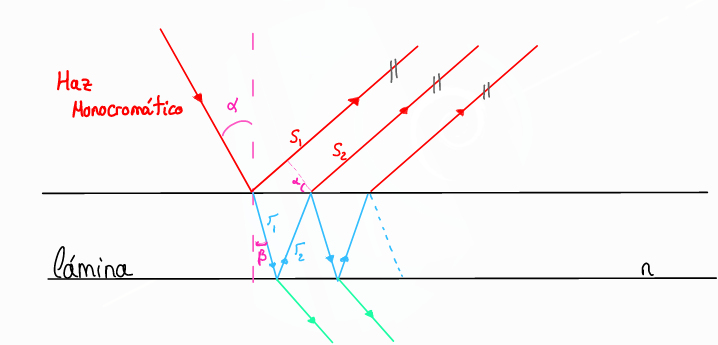
\includegraphics[width=0.5\textwidth]{imagen/diagramalamina.png}
	\caption{\small Representación del fenómeno de reflexión externa y externa del haz monocromático sobre la lámina y rayos que se emiten en el exterior de esta}
\end{figure}
donde $\alpha$ es el ángulo del rayo incidente y $\beta$ el reflejado respecto a la normal. Los rayos 
\\

El montaje queda representado por la figura %INTRODUCIR REFERENCIA DE FIGURA IPAD 2
donde $L$ es la distancia del foco virtual a la lámina. $r_m$ la medida de los radios, $d_{l-p}$ distancia lámpara pantalla y $d_{f-l}$ distancia foco virtual a la pantalla. Esta última medida la podemos obtener de manera directa midiendo la distancia de la lámpara a la lámina delgada, ya que el foco virtual es simétrico respecto al foto real (es decir, las distancias entre focos son iguales).
%% 				FIGURA IPAD 2
\begin{figure}[H]
	\centering
	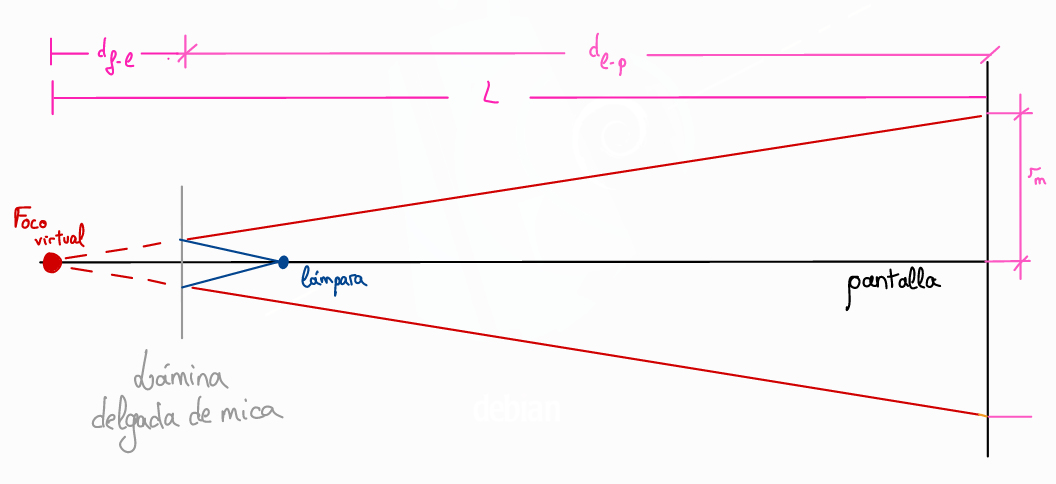
\includegraphics[width=0.5\textwidth]{imagen/diagramaexp.png}
	\caption{\small Esquema del método operativo junto con las variables indicadas.}
\end{figure}
\subsection{Tipos de variable }
A continuación clasificamos las variables obtenidas directamente en el laboratorio según si son variables dependientes, independientes o de control
\begin{itemize}
	\item {\textbf{Variables independientes:  }}
	\begin{itemize}
		\item Distancia placa-pantalla ($d_{l-p}$) y filtro placa ($d_{f-l}$)
		\item Valor de $\lambda, n,$ y $d$ cuando las tomamos como parámetros dados, en caso contrario debemos de tomarlas como variables dependientes según la ecuación:
			\begin{equation}
				m\lambda=2nd-\frac{d}{n}\sin^2 \alpha
				\label{orden}
			\end{equation}
	\end{itemize}

	\item{\textbf{Variables dependientes: }} 
		\begin{itemize}
			\item $L=L(d_{f-l}, d_{l-p})$ 
			\item $R_{ext}$ y $R_{int}$ dependen tanto de $\lambda, n$ y $m$ según la ecuación 1 siendo $m$ el orden de interferencia del anillo 
		\end{itemize}
	\item{\textbf{Variables de control}}
		\begin{itemize}
			\item Ruído lumínico del laboratorio: Al medir los radios externos e internos el ojo humano no puede evitar tener complicaciones cuando hay una intensidad de luz externa al experimento. Esto llevaría dificultades a la hora de medir la destrucción y construcción de la interferencia.
		\end{itemize}
\end{itemize}

\section{Resultados}%
Calculamos el valor de $L$ teniendo en cuenta los valores de las distancias medidas directamente.

 \[
	 d_{f-l}=\left( 75 \pm 1 \right) mm
.\] 
\[
	d_{l-p}=\left( 376 \pm 1 \right) mm
.\] 
Por tanto:
\[
	L=\left( 451\pm 2 \right) mm
.\] 
\subsection{Tabla de medidas directas}
A continuación representamos en tablas las medidas tomadas directamente del laboratorio para los radios externos e internos de cada filtro:
\begin{table}[H]
	\caption{Medidas de los radios interiores y exteriores obtenidos en el laboratorio para el filtro amarillo}
		\centering
	\begin{tabular}{|c|c|c|}
		\hline
		\rowcolor{yellow}
		\multicolumn{3}{|c|}{Filtro amarillo $\lambda= 580 $ nm} \\ \hline
		\pmb{	$m$} & \pmb{$R_{int} \pm 1 mm$} & \pmb{$R_{ext} \pm 1 mm$} \\ \hline
		$m_0-1/2$ & $72$ & $84$ \\ 
		$m_0 -1$ & $84$ & $92$ \\ 
		$m_0-3/2$ & $92$ & $103$ \\ 
		$m_0-2$ & $103$ & $111$ \\ 
		$m_0-5/2$ & $111$ &$ 121$ \\
		$m_0-3$ & $121$ & $128$ \\ 
		$m_0-7/2$ & $128$ & $136$ \\ \hline
	\end{tabular}
	\label{}
\end{table}


\begin{table}[H]
	\caption{Medidas de los radios interiores y exteriores obtenidos en el laboratorio para el filtro azul}
		\centering
	\begin{tabular}{|c|c|c|}
		\hline
		\rowcolor{cyan}
	\multicolumn{3}{|c|}{Filtro azul  $\lambda= 440 $ nm} \\ \hline
		\pmb{$m$} & \pmb{ $R_{int} \pm 1 mm$} & \pmb{$R_{ext} \pm 1 mm$} \\ \hline
		$m_0-1/2$ & $66$ & $79$ \\ 
		$m_0 -1$ & $79$ & $87$ \\ 
		$m_0-3/2$ & $87$ & $ 96$ \\
		$m_0-2$ & $96$ & $103$ \\
		$m_0-5/2$ & $103$ & $111$ \\ 
		$m_0-3$ & $111$ & $117$ \\ 
		$m_0-7/2$ & $117$ & $125$ \\ 
		$m_0 - 4$ & $125$ & $131$ \\ 
		$m_0 - 9/2$ & $131$ & $135$ \\ \hline
	\end{tabular}
	\label{}
\end{table}

% AZUL 2

\begin{table}[H]
	\caption{Medidas de los radios interiores y exteriores obtenidos en el laboratorio para el filtro verde}
		\centering
	\begin{tabular}{|c|c|c|}
		\hline
		\rowcolor{green}
		\multicolumn{3}{|c|}{Filtro verde $\lambda= 525 $ nm} \\ \hline
		\pmb{	$m$} & \pmb{$R_{int} \pm 1 mm$} & \pmb{$R_{ext} \pm 1 mm$} \\ \hline
		$m_0$ & $75$ & $85$ \\
		$m_0-1/2$ & $85$ & $99$ \\ 
		$m_0 -1$ & $99$ & $105$ \\ 
		$m_0-3/2$ & $105$ & $118$ \\ 
		$m_0-2$ & $118$ & $124$ \\ 
		$m_0-5/2$ & $124$ &$ 134$ \\
		$m_0-3$ & $134$ & $140$ \\ 
		$m_0-7/2$ & $140$ & $149$ \\ \hline
	\end{tabular}
	\label{}
\end{table}

\begin{table}[H]
	\caption{Medidas de los radios interiores y exteriores obtenidos en el laboratorio para el filtro desconocido}
		\centering
	\begin{tabular}{|c|c|c|}
		\hline
		\pmb{$m$} & \pmb{ $R_{int} \pm 1 mm$} & \pmb{$R_{ext} \pm 1 mm$} \\ \hline
		$m_0-1/2$ & $61$ & $74$ \\ 
		$m_0 -1$ & $74$ & $79$ \\ 
		$m_0-3/2$ & $79$ & $ 91$ \\
		$m_0-2$ & $91$ & $96$ \\
		$m_0-5/2$ & $96$ & $105$ \\ 
		$m_0-3$ & $105$ & $110$ \\ 
		$m_0-7/2$ & $110$ & $119$ \\ 
		$m_0 - 4$ & $119$ & $123$ \\ 
		$m_0 - 9/2$ & $123$ & $130$ \\ \hline
	\end{tabular}
	\label{}
\end{table}


\subsection{Gráficas y resultados}
Para hallar los valores que nos piden, usaremos la fórmula (1) para hacer una estimación lineal, teniendo como pendiente la variable a estudiar, utilizando las demás variables como variables conocidas para nuestro estudio concreto
\subsubsection{Obtención de $d$ a través de mínimos cuadrados}
Datos conocidos: $\lambda=( 580 \pm 1) nm$ , $n=1.6\pm 0.1$\
Mediante la fórmula (1) obtendremos el valor de $d$, siendo esta 
$d=d(\lambda,n,sin^2 \alpha,m)$ mediante los valores obtenidos del laboratorio para el filtro amarillo\\
\\
La tabla con los valores de cada variable y su error junto con el método de mínimos cuadrados se encuentran en el Anexo (1)\\
\\
Representando gráficamente para obtener una regresión lineal cuya pendiente sea $d$ :
\begin{figure}[H]
	\centering
	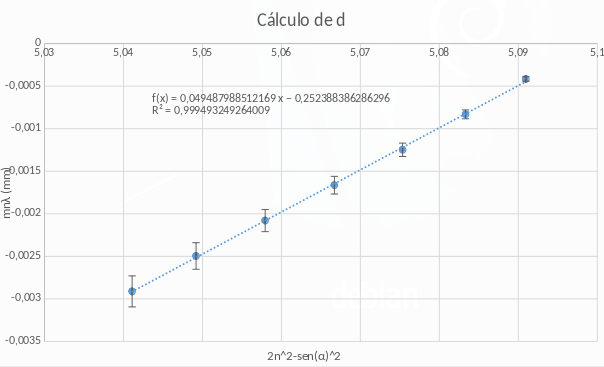
\includegraphics[width=0.50\textwidth]{imagen/graficad.png}
	\caption{Representación gráfica para la obtención de $d$}
	\label{fig:imagen-}
\end{figure}
El valor de $d$ obtenido por tanto, es :
\begin{equation}
	\boxed{d=(49.5 \pm 5) micras}
\end{equation}
\subsubsection{Obtención de $n$ a través de mínimos cuadrados usando el filtro verde}
Datos conocidos: $\lambda=525\pm 1 nm$, $d=(32 \pm 1$) micras \\

La tabla de datos se encuentra en la tabla de Anexo (2). La gráfica obtenida para representar el valor de $n$ como pendiente se encuentra en la figura (4):
\begin{figure}[H]
	\centering
	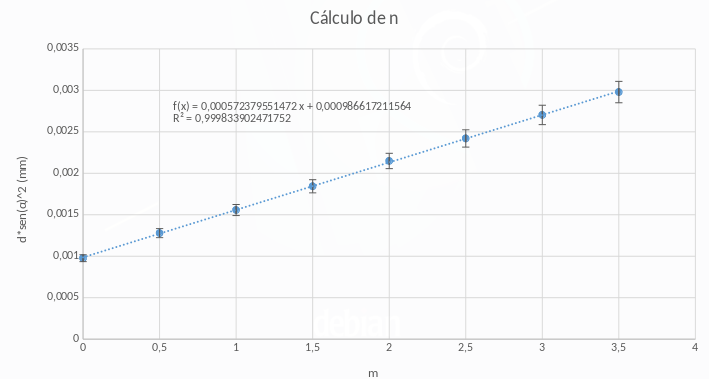
\includegraphics[width=0.5\textwidth]{imagen/grafican.png}
	\caption{Representación gráfica para obtener $n$ mediante el filtro verde}
	\label{fig:imagen-}
\end{figure}
El valor obtenido con la estimación lineal no es de por si el valor de $n$, sino que viene dado por:
\[
n=\frac{p}{\lambda}
.\] 
donde $p$ es la pendiente de la recta regresión. El error lo calculamos mediante:
\[
	\Delta n=\sqrt{\left( \frac{\partial n}{\partial \lambda}  \right) ^2 \left( \Delta \lambda \right) ^2+ \left( \frac{\partial n}{\partial p}  \right) ^2 \left( \Delta p \right) ^2} 
.\] 
Con todo ello, el valor de $n$ es :
\begin{equation}
	\boxed{n=\left( 1.09 \pm 0.9 \right) }
\end{equation}
\subsubsection{Obtención de $\lambda$ usando el filtro azul }
Datos conocidos: $d=(32 \pm 1 $) micras,  $n=1,6 \pm 1$\\
A partir de los datos conocidos usando la tabla de datos del filtro azul, usamos la fórmula (1) para realizar una estimación lineal de los datos, donde nuestra pendiente es  $\lambda$.\\
\\
Los cálculos del método de mínimos cuadrados junto con sus errores se encuentran en el Anexo (3)




\begin{figure}[H]
	\centering
	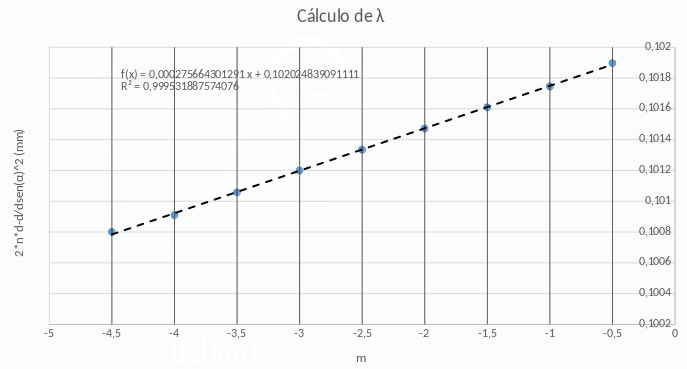
\includegraphics[width=0.50\textwidth]{imagen/grafical1.png }
	\caption{Representación gráfica de la estimación lineal para el cálculo experimental de $\lambda$ para el filtro azul}
	\label{fig:imagen-grafical1-png-}
\end{figure}

%%% 				GRÁFICA OBTENCIÓN LAMBDA AZUL



El valor hallado para $\lambda$ es de:
\begin{equation}
	\boxed{\lambda=\left( 276 \pm 3  \right) nm}
\end{equation}
\subsubsection{Obtención de $\lambda$ para el filtro desconocido}
Datos conocidos: $d=(32\pm 1$) micras , $n=1,6 \pm 1$ \\
Hallamos $\lambda$ al igual que el punto anterior, calculando la pendiente mediante regresión lineal con los valores de la tabla de datos medidos directamente para el filtro desconocido.\\
\\
La tabla donde se encuentran los cálculos del método de mínimos cuadrados se encuentran en el Anexo (4).

\begin{figure}[H]
	\centering
	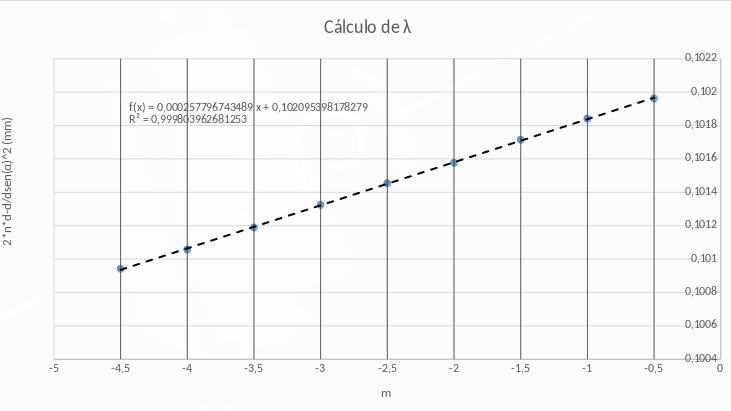
\includegraphics[width=0.51\textwidth]{imagen/grafical2.png}
	\caption{Representación gráfica de la estimación lineal para el cálculo de $\lambda$}
\end{figure}
%%% 				GRÁFICA OBTENCIÓN LAMBDA DESCONOCIDO

El valor de $\lambda$ desconocido es:

\begin{equation}
	\boxed{\lambda=\left( 257.9 \pm 1.8 \right) nm}
\end{equation}
\section{Discusión}%
\label{sec:i}
 Los valores obtenidos para el espesor de la lámina de micra es:

\begin{equation}
	\boxed{d=(49.5 \pm 0.5) micras}
\end{equation}
El valor teórico del espesor es de $d=32$ micras. Nuestro valor experimental no es compatible con el valor teórico. No obtenemos este valor ni aunque aumentáramos el valor del error a más de lo que podemos para deducir que ha sido un fallo estadístico. El erro relativo teórico es de $e=54\%$. Un valor bastante alto para nuestros intereses.\\
\\
Al hallar el valor del índice de refracción del medio nos sale:

\begin{equation}
	\boxed{n=\left( 1.09 \pm 0.09 \right) }
\end{equation}
El valor teórico de esta variable es $n=(1.6 \pm 0.1)$, siendo por tanto el valor relativo del  $31\%$. Esto nos vuelve a indicar que la medida es bastante inexacta a la par de incompatible con el resultado teórico. \\
\\
El valor de la longitud de onda del filtro azul es de 

\begin{equation}
	\boxed{\lambda=(275\pm 3)nm}
\end{equation}

siendo el valor teórico del filtro azul de $\lambda=(525\pm 1)$ nm. El error teórico es, por tanto del 37\%

Por último, observamos que el valor calculado para el filtro desconocido es de 

\begin{equation}
	\boxed{\lambda=\left( 257.9 \pm 1.8 \right) nm}
\end{equation}
siendo el valor esperado de $\lambda=\left( 580\pm 1\right) nm$, correspondiendo este último valor a la longitud de onda del color morado. El valor experimental de nuevo se aleja del resultado teórico siendo el error relativo del 55\%.\\
\\
Los resultados obtenidos difieren de los esperados. Los datos, con su error, se alejan de los valores teóricos. La razón más plausible, es que el error humano es mayor de lo que inicialmente le habíamos asociado.\\
\\
El lugar en el proceso del experimento donde el error humano se hace más notable es al determinar la frontera que separa lo que es un 'máximo' y un 'mínimo'.\\
\\
A ojo, determinábamos esa posición, en un papel milimitrado, cuya sensibilidad es de un milímetro. Tendríamos que haber aumentado la magnitud del error en esa medida, al aumentar el error humano. De todos modos, los órdenes de las magnitudes de los datos obtendos y los teóricos coinciden.
\section{Conclusión}%
La datos finales de la práctica son del orden de los datos teóricos, pero no son compatibles. A pesar de ésto, hemos experimentado de cualitativamente y, de forma orientativa, cuantitativamente los fenómenos de interferencia de la luz. Teniendo en cuenta todo esto (y que además, vimos la sombra de una aguja ese día), estamos satisfechos con la práctica.
\begin{thebibliography}{0}
	\bibitem{tapetum} \href{https://en.wikipedia.org/wiki/Tapetum_lucidum}{\textcolor{blue}{Tapetum lucidum. Wikipedia }} 
\end{thebibliography}

\onecolumn
\section{Anexo}%
\begin{itemize}
	\item (1): 
		\begin{figure}[H]
			\centering
			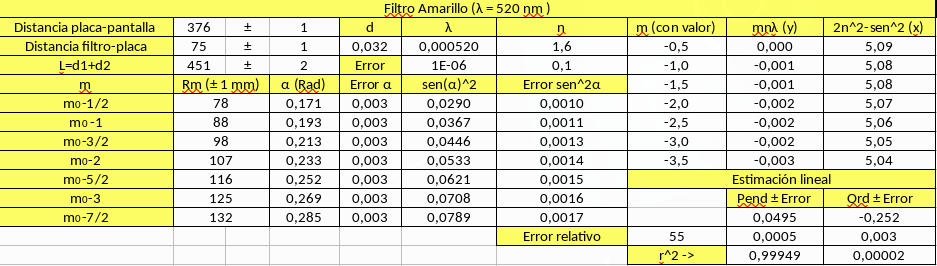
\includegraphics[width=0.9\textwidth]{imagen/anexo1.png}
			\caption{Método de mínimos cuadrados, variables y errores calculados}
			\label{fig:imagen-}
		\end{figure}

	\item (2): 
		\begin{figure}[H]
			\centering
			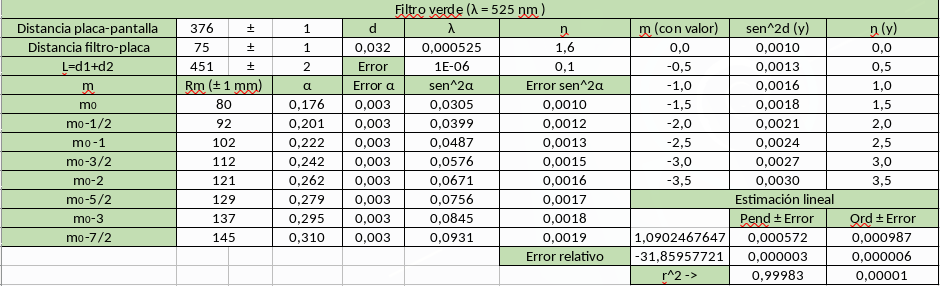
\includegraphics[width=0.9\textwidth]{imagen/anexo2.png}
			\caption{Método de mínimos cuadrados, variables y errores calculados}
			\label{fig:imagen-}
		\end{figure}

	\item (3): 
		\begin{figure}[H]
			\centering
			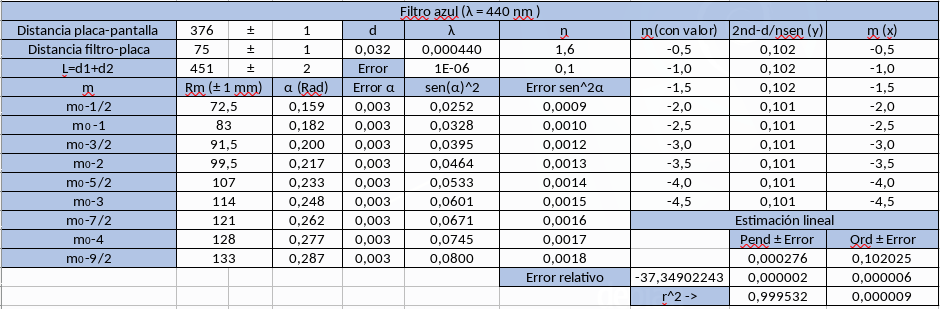
\includegraphics[width=0.9\textwidth]{imagen/anexo3.png}
			\caption{Método de mínimos cuadrados, variables y errores calculados}
			\label{fig:imagen-}
		\end{figure}
\newpage
	\item (4): 
		\begin{figure}[H]
			\centering
			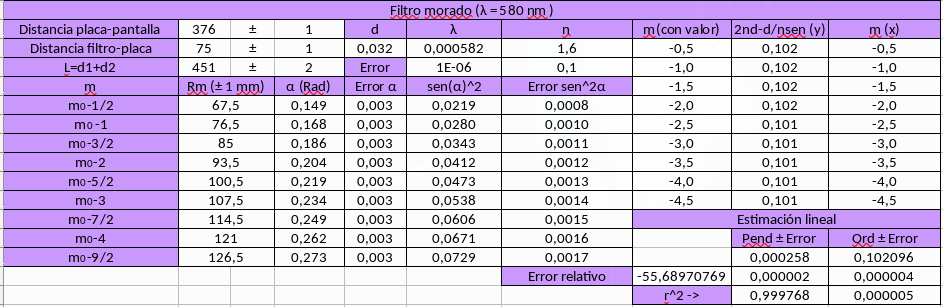
\includegraphics[width=0.9\textwidth]{imagen/anexo4.png}
			\caption{Método de mínimos cuadrados, variables y errores calculados}
			\label{fig:imagen-}
		\end{figure}
\end{itemize}
\end{document}
